\subsection{System Model}\label{sec:application:cloud_file_synchronisation:system_model}
\subsubsection*{Use Case: Photo Uploading}\label{sec:application:cloud_file_synchronisation:use_case}
In this section we consider the synchronization of images from a digital camera to a mobile \gls{UE} via a cloud storage provider.
Real world examples of this scenario are, e.g., taking photos of a live event and transferring them to a picture agency, or shooting private holiday images. 

The user took a finite set of pictures with a wearable device like Google Glass or a smart camera, e.g. a Nikon Coolpix S800c or SAMSUNG CL80.
The camera is then connected via a \gls{PAN} with a mobile \gls{UE}, for example a Laptop with a data card or a smart phone, to store the images on the mobile device.
The \gls{UE} uses broadband wireless Internet access technology and runs software provided by the cloud storage provider in order to synchronise the images with the cloud storage.
Finally, the scenario includes a remote client, which is connected using a wire line connection and downloads the images from the cloud.

For the evaluation presented in this paper, we consider a specific realization of the use case described above.
For the role of the cloud storage provider we consider \dropbox, Bluetooth is used as the technology for establishing the \gls{PAN}, and \gls{LTE} is used as the wireless broadband access technology.

In the considered scenario the interests of two stakeholders are impacted.
The first stakeholder, the end user, has two contradicting requirements on the system.
On the one hand side, the images should be synchronised as fast as possible. 
This requires a fast and permanent Internet connection of the \gls{UE}, which in turn is very power intensive.
On the other side, the energy consumption of the mobile device should be minimized to enable a long battery life time.
The second stakeholder, the mobile network provider, wants to minimize the signalization overhead in the network~\cite{NSN2011, Huawei2011} caused by short time connections.
Here, an optimization problem arises to find a practical solution for all three requirements. 
In order to analyse this problem, we use a simulation model of the file synchronization process, which is described in the following.

\subsubsection*{Cloud Storage Model and Performance Metrics}\label{sec:application:cloud_file_synchronisation:system_model:model_metrics}
The proposed simulation model is schematically depicted in \reffig{fig:application:cloud_file_synchronisation:system_model:model_metrics:model} and based on the findings of~\cite{drago2012} described in~\refsec{sec:application:background}.

\begin{figure}
\centering
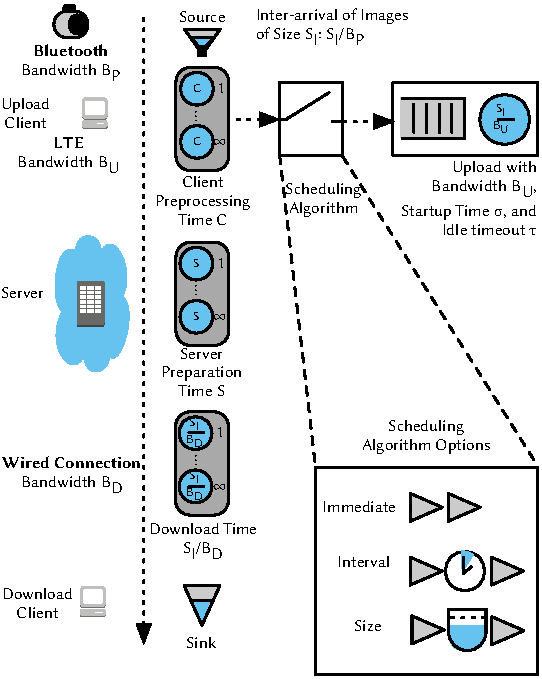
\includegraphics[width=\columnwidth]{application/cloud_file_synchronization/system_model/figures/model}
\caption{Synchronization Process Model}
\label{fig:application:cloud_file_synchronisation:system_model:model_metrics:model}
\end{figure}

We assume that the user has taken pictures of varying file size distributed with \imageFileSize.
These pictures are transfered from the camera to the mobile device using the \gls{PAN} with a constant bandwidth~\panTransferRate.
Due to the limited bandwidth \panTransferRate of the \gls{PAN} device, the inter-arrival times of images at the \dropbox shared folder of the mobile device can be calcluated by \(\interarrivaltime = \frac{\imageFileSize}{\panTransferRate}\).

As soon as the image is fully copied to the \dropbox folder, the generation of the meta data introduces a preprocessing delay, which we refer to as client preparation time~\clientpreparationtime.
To evaluate different strategies optimising the overall waiting time, energy consumption, and signalisation traffic we include a scheduling component.
This component implements different algorithms, described in \refsec{sec:application:cloud_file_synchronisation:system_model:algorithms}, which decide when the images currently held available in the scheduling component should be sent to the component responsible for transmission.

Next, we consider the \gls{LTE} \gls{UE} used for image upload.
Due to the specification of the \gls{LTE} standard \cite{3GPP_RRC_Spec}, the upload component can, at any point in time, either be connected to the mobile network or disconnected.
If the \gls{UE} is currently disconnected, and a new image for upload arrives, the connection process is triggered and completed after a startup delay \(\startupDelay = \SI{0.26}{\second}\).
Once the \gls{UE} is connected, arriving images are transmitted in order.
The transmission, i.e. service time, of an image depends on the size of the image currently being uploaded as well as the upload bandwidth \uploadbandwidth.
As only one image is transferred at once, waiting images are stored in a queue of infinite size.
If the \gls{UE} is idle for more than \(\idleThreshold = \SI{11.576}{\second}\), the device disconnects from the network.

After the image has been successfully uploaded to the storage servers, a server side preprocessing phase starts, before the file transfer to the downloading client starts.
This server side preprocessing again introduces an additional delay, the server preparation time~\serverpreparationtime, in the synchronization process.
Finally, the image is downloaded by the wire line client.
Again, the duration is calculated based on the size of the image and the available download bandwidth~\downloadbandwidth.

Next, we discuss the metrics used to evaluate the performance of the scheduling algorithms under consideration.
First, we consider the mean synchronization time \sojournTime, i.e., the time between the generation of images and the completion of the download.
This metric accounts for the desire of end users to synchronize images in a short amount of time.
Secondly, we study the relative amount of time the \gls{UE} is disconnected \relativeDisconnectedTime.
As the \gls{UE} consumes more power in the connected state, the user is generally interested in scheduling mechanisms which ensure that the device is only connected if required \cite{Ickin2012}.
This measure also enables a more general evaluation then the actually consumed energy, because the concrete energy consumption differs significantly for each device.
Finally, we evaluate the number of transitions~\connectionCount between the connected and disconnected states.
As discussed in \refsec{chap:network}, frequent state transitions put a strain on the network due to increased signalling.
Thus, scheduling algorithms with a small number of transitions would be favored by network operators.

\subsubsection*{Scheduling Algorithms}\label{sec:application:cloud_file_synchronisation:system_model:algorithms}
We use different scheduling strategies in our model to control the uploading of the files from the mobile client.
These mechanisms in turn affect the synchronization time, the energy consumption, and the generated signaling traffic.

The most basic strategy of handing the upload is to immediately send new files, as soon as the meta data is generated.
We refer to this as \algoimmediate strategy and will use this as base line for all comparisons in the evaluations.
The other two strategies considered are based on a temporal, respectively a size threshold. 
Using the \algointerval scheduling, the client checks periodically if new files have been marked for synchronization.
If new files are present, they are synchronized to \dropbox.
Files which could not be sent within the current interval will automatically be added to the file batch for the next interval. 
The last scheduling mechanisms uses a threshold based on the overall \algosize of the images not yet synchronized.
If the threshold is crossed, an upload is triggered.
